% ============================================================================
%  Vortex street -- a from-scratch incompressible Navier-Stokes solver,
%  benchmark-verified and inverted into a flow-meter.
%  Technical report -- B.Sc. Computational Engineering Science (CES), RWTH Aachen
%
%  COMPILE: upload this folder (report.tex + figures/) to Overleaf, "Recompile"
%  (pdfLaTeX). Locally: pdflatex report.tex (run twice).
% ============================================================================
\documentclass[11pt,a4paper]{article}

\usepackage[T1]{fontenc}
\usepackage[utf8]{inputenc}
\usepackage{lmodern}
\usepackage[margin=2.3cm]{geometry}
\usepackage{amsmath,amssymb}
\usepackage{graphicx}
\usepackage{booktabs}
\usepackage{siunitx}
\usepackage{caption}
\usepackage{subcaption}
\usepackage[hidelinks]{hyperref}
\usepackage{xcolor}
\usepackage{enumitem}

\sisetup{detect-all}
\graphicspath{{figures/}}
\captionsetup{font=small,labelfont=bf}
\setlist{nosep,leftmargin=1.4em}

% --- RWTH house colours + banner -------------------------------------------
\definecolor{rwthblue}{HTML}{00549F}
\definecolor{rwthblue25}{HTML}{C7DDF2}
\definecolor{rule}{HTML}{8EBAE5}
\newcommand{\rwthbanner}{%
  \noindent\colorbox{rwthblue}{%
    \parbox{\dimexpr\textwidth-2\fboxsep\relax}{%
      \vspace{2.5pt}%
      {\color{white}\textbf{RWTH AACHEN UNIVERSITY}}\hfill
      {\color{white}\footnotesize Computational Engineering Science}%
      \vspace{2.5pt}}}%
  \vspace{1pt}\par\noindent{\color{rule}\rule{\textwidth}{1.3pt}}%
}

\begin{document}

% ---- title block -----------------------------------------------------------
\rwthbanner
\vspace{0.8em}

{\raggedright
  {\LARGE\bfseries The von K\'arm\'an vortex street}\\[0.35em]
  {\large A from-scratch incompressible Navier--Stokes solver, benchmark-verified\\
   and inverted into a flow-meter}\\[0.8em]
  {\normalsize Muhammet Emir Fil}\\[0.15em]
  {\small B.Sc.\ Computational Engineering Science, RWTH Aachen \quad\textbullet\quad Technical report, \today}\par
}
\vspace{0.6em}
\noindent{\color{rule}\rule{\textwidth}{0.6pt}}
\vspace{1.0em}

% ---- AIM -------------------------------------------------------------------
\noindent\colorbox{rwthblue25}{%
  \parbox{\dimexpr\textwidth-2\fboxsep\relax}{%
  \vspace{3pt}\textbf{Aim.} Write a 2D incompressible Navier--Stokes solver from scratch, verify
  it against canonical benchmarks, and then invert it into a vortex flow-meter that reads the flow
  speed from the wake frequency. The goal is a forward PDE solver trustworthy enough to be used
  backwards as a measurement, with the finite-domain error reported rather than tuned away. The
  core is numpy-only and every result ships with the reference it was checked against.\vspace{3pt}}}

\vspace{1.0em}

\begin{abstract}
\noindent
A 2D incompressible Navier--Stokes solver is written from scratch in numpy on a staggered (MAC)
grid with Chorin projection, and used to model flow past a cylinder: the steady recirculation
bubble, the von K\'arm\'an vortex street, and vortex-induced vibration (VIV) lock-in of an
elastically mounted cylinder. The solver is verified against four classical benchmarks (Ghia et
al.\ lid-driven cavity; Coutanceau--Bouard wake length; Williamson shedding Strouhal number;
Khalak--Williamson VIV amplitude). It is then inverted: because a bluff body sheds at
$f=\mathrm{St}\,U/D$, the wake frequency reads back the free-stream speed, which makes a vortex
flow-meter, demonstrated as a simulate-then-recover round trip with a Monte-Carlo confidence
interval. Finite-domain blockage shifts the force coefficients above their unbounded references;
the offset is reported rather than tuned away, and cancels in the calibrated inverse.
\end{abstract}

% ---------------------------------------------------------------------------
\section{Motivation}
% ---------------------------------------------------------------------------
The same wake that makes a flag flutter and a chimney resonate is a clock: a bluff body in a steady
stream sheds vortices at a frequency proportional to the flow speed. Building the solver that
produces that wake from first principles, and then running it backwards to read the speed off the
shedding frequency, exercises the full computational pipeline: discretising the incompressible
Navier--Stokes equations, enforcing the divergence-free constraint, representing a solid body on a
regular grid, validating against canonical benchmarks, and turning a verified forward model into a
measurement. The core is numpy-only and every result ships with the reference it was checked
against.

% ---------------------------------------------------------------------------
\section{Method (forward solver)}
% ---------------------------------------------------------------------------
\paragraph{Governing equations.} The incompressible Navier--Stokes equations,
\begin{equation}
  \frac{\partial \mathbf{u}}{\partial t} + (\mathbf{u}\cdot\nabla)\mathbf{u}
  = -\nabla p + \nu\nabla^2\mathbf{u},\qquad \nabla\cdot\mathbf{u}=0,
  \label{eq:ns}
\end{equation}
are discretised on a staggered MAC grid (pressure at cell centres, velocities at face midpoints),
which avoids the odd--even pressure decoupling of a collocated grid.

\paragraph{Projection.} Time advance uses Chorin's projection method: an intermediate velocity
$\mathbf{u}^\star$ is formed from advection and diffusion, then projected onto the divergence-free
space by solving the pressure Poisson equation
$\nabla^2 p = \tfrac{1}{\Delta t}\nabla\cdot\mathbf{u}^\star$. On the regular grid this is solved
spectrally with a discrete cosine transform, which is fast and exact to round-off and keeps the
iterative-solver cost out of the inner loop.

\paragraph{Immersed cylinder.} The cylinder is represented by volume penalisation: a penalty term
drives the velocity to zero inside the solid, and the integrated penalty reaction is the
hydrodynamic force on the body (drag and lift), so the force coefficients come out of the same
field that enforces the boundary. On a spring, the cylinder's transverse equation of motion is
integrated alongside the flow, giving two-way fluid--structure coupling (VIV).

% ---------------------------------------------------------------------------
\section{Verification against benchmarks}
% ---------------------------------------------------------------------------
The solver is checked against four classical results spanning the regimes it claims
(Table~\ref{tab:verify}).

\begin{table}[h]
  \centering
  \caption{Verification against canonical CFD benchmarks.}
  \label{tab:verify}
  \footnotesize
  \setlength{\tabcolsep}{4pt}
  \begin{tabular}{@{}llll@{}}
    \toprule
    Check & This solver & Reference & \\
    \midrule
    Lid-driven cavity centreline $u,v$ (Re 100) & RMS $2.2/4.5\times10^{-3}$ & Ghia, Ghia \& Shin 1982 & ok \\
    Steady wake bubble $L_w/D$ (Re 20 / 40)      & 0.88 / 2.03               & 0.93 / 2.24 (Coutanceau--Bouard) & ok \\
    Shedding Strouhal $\mathrm{St}$ (Re 100)     & 0.18                      & 0.16 unbounded (Williamson 1988) & $+$ blockage \\
    Drag / lift $C_d,C_l$ (Re 100)               & 1.56 / 0.42               & $\sim$1.33 / $\sim$0.33 unbounded & $+$ blockage \\
    VIV lock-in peak $A/D$                        & $\approx 0.5$--$0.6$      & Khalak \& Williamson 1999 & ok \\
    \bottomrule
  \end{tabular}
\end{table}

The lid-driven cavity is the decisive correctness test: the centreline velocity profiles match the
Ghia et al.\ (1982) tabulated data to RMS of order $10^{-3}$ (Fig.~\ref{fig:bench}, left), which
confirms the advection, diffusion, and projection are all right. The steady wake length and the VIV
lock-in amplitude validate the immersed body and the fluid--structure coupling against the
experimental literature.

\paragraph{Blockage, reported not tuned.} A finite domain confines the flow, raising
$\mathrm{St}$, $C_d$, and $C_l$ above their unbounded references. This offset is quantified
($\mathrm{St}$: 0.20 at 17\,\% blockage, 0.18 at 8\,\%, toward 0.16 as the walls recede) rather than
fitted away, which is the honest way to present a finite-domain solver.

\begin{figure}[h]
  \centering
  \begin{subfigure}{0.48\textwidth}
    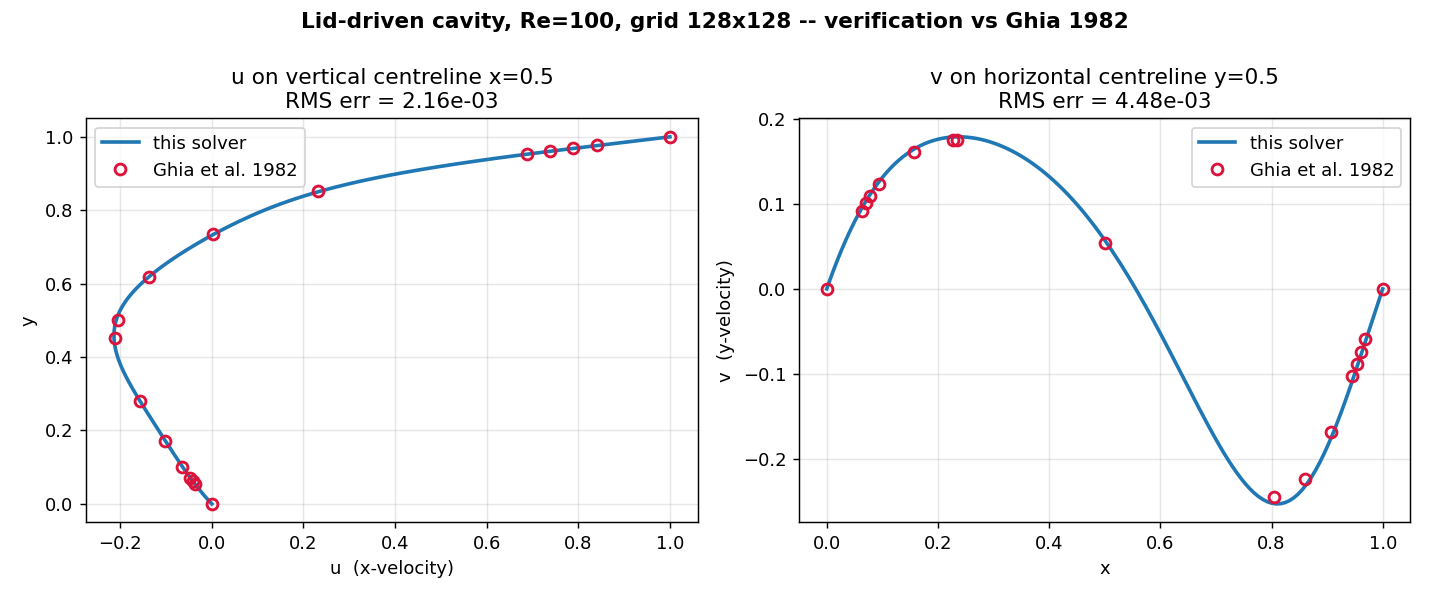
\includegraphics[width=\linewidth]{cavity_ghia_Re100.png}
    \caption{Lid-driven cavity centreline profiles vs Ghia et al.\ 1982.}
  \end{subfigure}\hfill
  \begin{subfigure}{0.48\textwidth}
    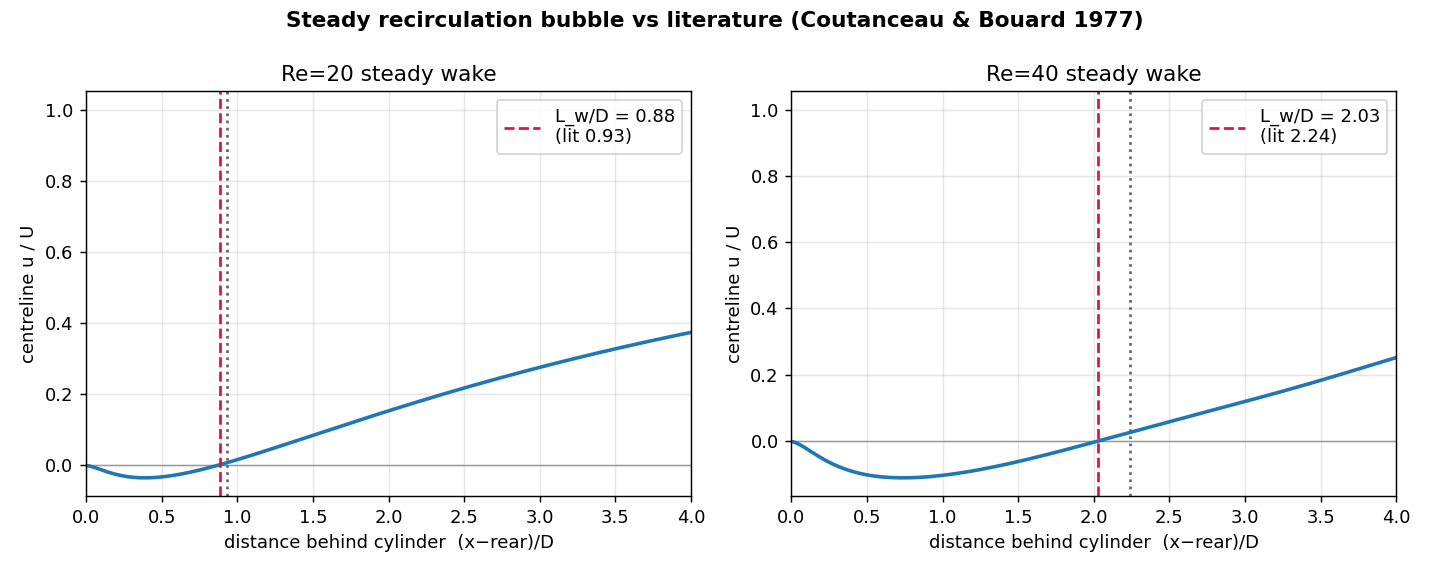
\includegraphics[width=\linewidth]{cylinder_steady.png}
    \caption{Steady recirculation bubble; length vs Coutanceau--Bouard.}
  \end{subfigure}
  \caption{Verification: the decisive cavity benchmark (left) and the steady wake (right).}
  \label{fig:bench}
\end{figure}

% ---------------------------------------------------------------------------
\section{The vortex street and VIV}
% ---------------------------------------------------------------------------
Above $\mathrm{Re}\approx 47$ the wake becomes unstable and sheds the periodic von K\'arm\'an
vortex street (Fig.~\ref{fig:street}, left). When the cylinder is mounted on a spring, the
alternating lift locks onto the structural frequency over a band of reduced velocities
(vortex-induced vibration lock-in), and the amplitude rises to $A/D\approx 0.5$--$0.6$ at the peak
(Fig.~\ref{fig:street}, right), consistent with the Khalak--Williamson experiments. This is the
mechanism behind oscillating chimneys, risers, and heat-exchanger tubes.

\begin{figure}[h]
  \centering
  \begin{subfigure}{0.62\textwidth}
    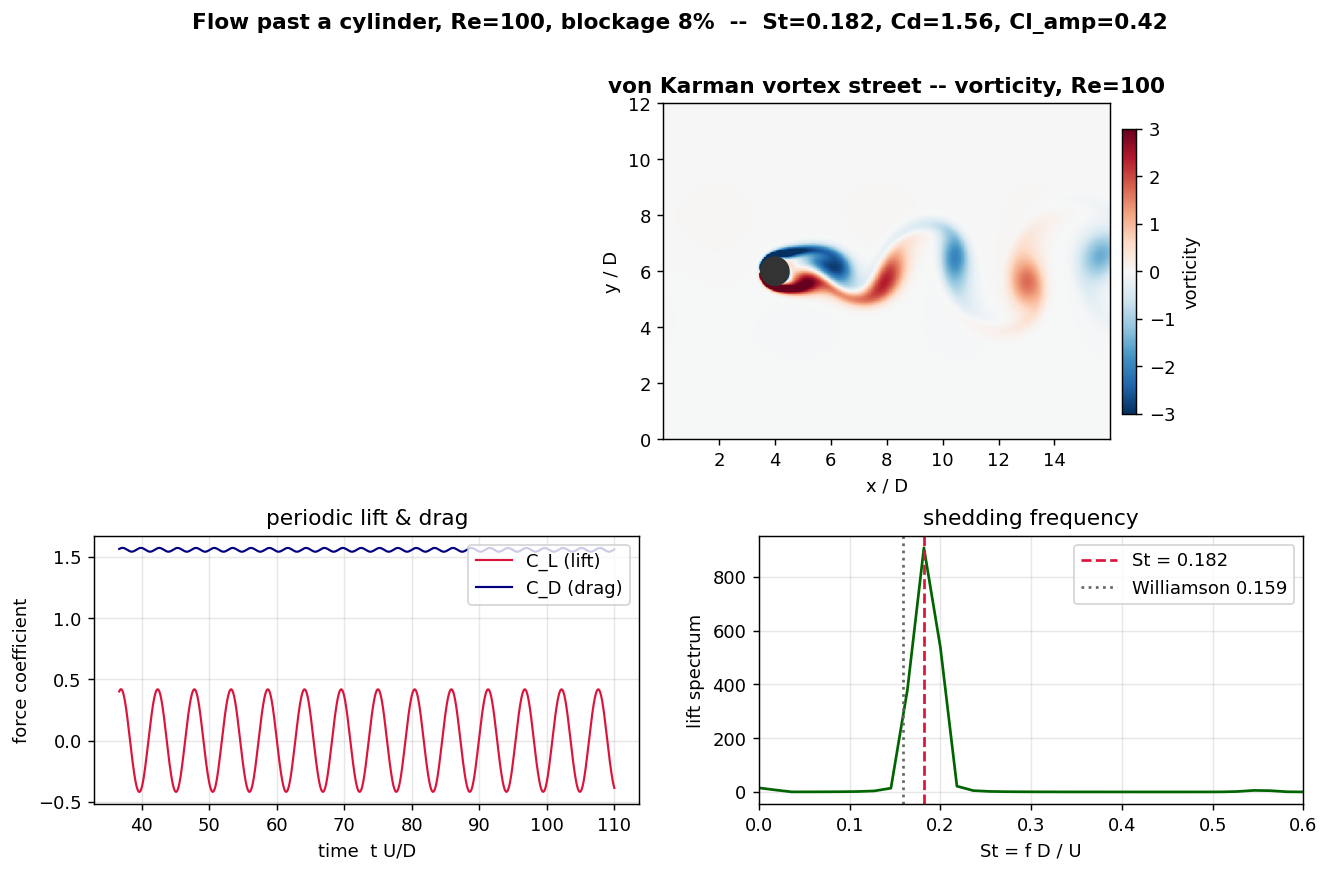
\includegraphics[width=\linewidth]{cylinder_Re100.png}
    \caption{Von K\'arm\'an vortex street, vorticity field at Re\,=\,100.}
  \end{subfigure}\hfill
  \begin{subfigure}{0.36\textwidth}
    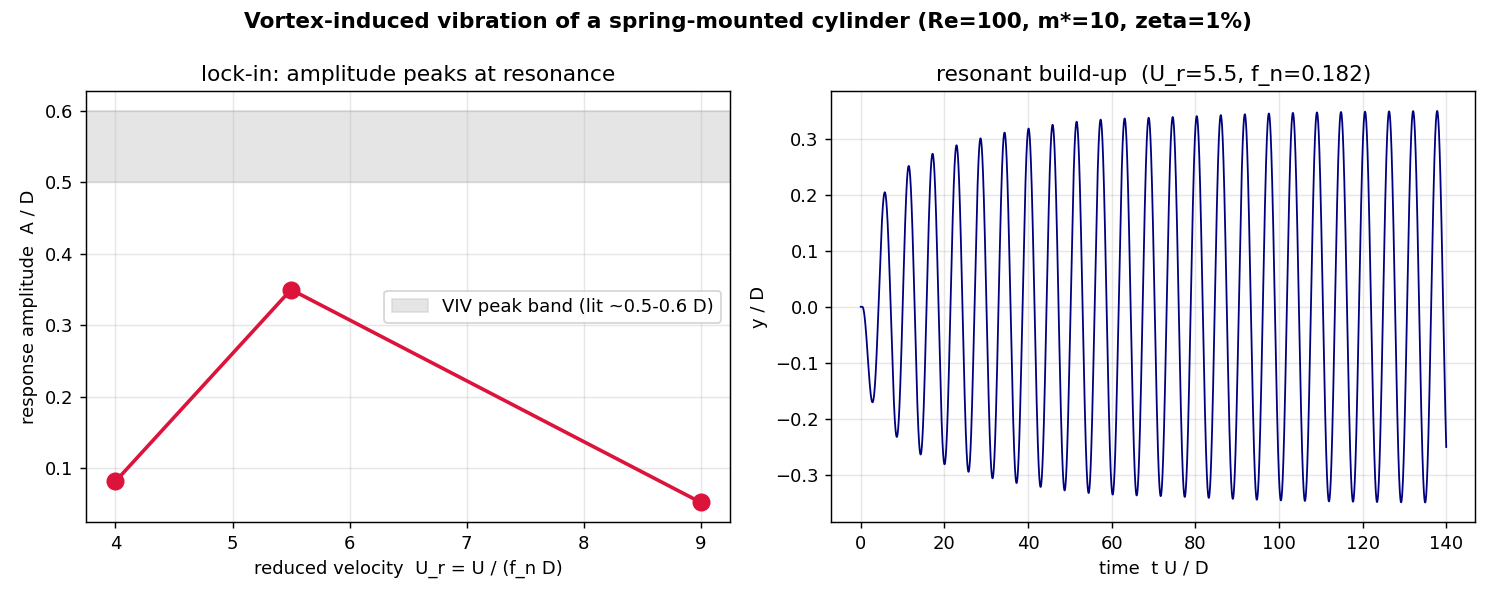
\includegraphics[width=\linewidth]{viv_lockin.png}
    \caption{VIV lock-in amplitude vs reduced velocity.}
  \end{subfigure}
  \caption{The shedding wake (left) and the fluid--structure lock-in it drives (right).}
  \label{fig:street}
\end{figure}

% ---------------------------------------------------------------------------
\section{Inversion: a vortex flow-meter}
% ---------------------------------------------------------------------------
A bluff body sheds at $f = \mathrm{St}(\mathrm{Re})\,U/D$, so the wake frequency is a direct
read-out of the flow speed, which is the principle of an industrial vortex flow-meter. The verified
forward solver is inverted to demonstrate it: for a known free-stream $U$ the solver sheds at $f$;
reading $f$ from the (noise-added) lift signal and inverting the solver-calibrated
$\mathrm{St}(\mathrm{Re})$ relation recovers $U$, with a 95\,\% confidence interval from a
sensor-noise Monte-Carlo. Because the same $\mathrm{St}(\mathrm{Re})$ is used forwards and
backwards, the finite-domain blockage cancels in the round trip, exactly the way a real meter is
calibrated per device. This closes the forward-to-inverse loop: a from-scratch PDE solver,
validated against benchmarks, then used as a measurement instrument with quantified uncertainty.

% ---------------------------------------------------------------------------
\section{Limitations}
% ---------------------------------------------------------------------------
\begin{itemize}
  \item 2D and laminar (Re up to a few hundred); a single circular cylinder.
  \item Volume penalisation gives $\mathcal{O}(\sqrt{\eta})$ boundary accuracy and a slightly
        thick effective cylinder.
  \item Finite-domain blockage shifts the force coefficients (quantified above; it cancels in the
        calibrated inverse).
  \item Explicit time stepping caps the step (CFL and diffusive stability).
\end{itemize}

% ---------------------------------------------------------------------------
\section{Reproducibility}
% ---------------------------------------------------------------------------
\begin{sloppypar}
The core is numpy-only. Each result is reproduced by a script that prints its numbers and saves the
figure shown here: \texttt{verify\_cavity.py} (Ghia 1982), \texttt{verify\_cylinder.py} (vortex
street, $\mathrm{St}/C_d/C_l$), \texttt{verify\_cylinder\_steady.py} (wake length),
\texttt{verify\_viv.py} (lock-in), and \texttt{verify\_flowmeter.py} (the inverse recovery and CI).
An interactive web demo animates a live vortex street with data injected (no server).
\end{sloppypar}

% ---------------------------------------------------------------------------
\begin{thebibliography}{9}
\small
\bibitem{ghia} U.\ Ghia, K.\,N.\ Ghia \& C.\,T.\ Shin, ``High-Re solutions for incompressible flow
  using the Navier--Stokes equations and a multigrid method,'' \emph{J.\ Comput.\ Phys.}, 48, 1982.
\bibitem{chorin} A.\,J.\ Chorin, ``Numerical solution of the Navier--Stokes equations,''
  \emph{Math.\ Comp.}, 22, 1968. (The projection method.)
\bibitem{williamson} C.\,H.\,K.\ Williamson, ``Vortex dynamics in the cylinder wake,''
  \emph{Annu.\ Rev.\ Fluid Mech.}, 28, 1996; Strouhal--Reynolds relation (1988).
\bibitem{coutanceau} M.\ Coutanceau \& R.\ Bouard, steady wake recirculation length behind a
  circular cylinder, \emph{J.\ Fluid Mech.}, 79, 1977.
\bibitem{khalak} A.\ Khalak \& C.\,H.\,K.\ Williamson, ``Motions, forces and mode transitions in
  vortex-induced vibrations at low mass-damping,'' \emph{J.\ Fluids Struct.}, 13, 1999.
\bibitem{angot} P.\ Angot, C.-H.\ Bruneau \& P.\ Fabrie, ``A penalization method to take into
  account obstacles in incompressible viscous flows,'' \emph{Numer.\ Math.}, 81, 1999.
\end{thebibliography}

\end{document}
